\documentclass{article}
\usepackage[utf8]{inputenc}
\usepackage{graphicx}


\title{RestaurantManager}
\author{Bella(1942308), De Persio(1938022)}
\date{}
\begin{document}

\maketitle

\section{Introduzione}

    Questo progetto da noi sviluppato consiste in un applicativo per la gestione di un ristorante che permette ai vari dipendenti di svolgere le loro mansioni principali e di scambiarsi informazioni utili a quest'ultime. \\
    Il lavoro ha subito varie ripartizioni a causa dell'abbandono di un nostro collega ma abbiamo comunque diviso lo sviluppo ordinatamente.
    \par Il progetto è stato ripartito nel modo seguente:
    \begin{itemize}
        \item Lo sviluppo della GUI
        \item Sviluppo backend              %MODIFICA
    \end{itemize}


\section{Descrizione delle Classi}

    \subsection{Interfaccia Grafica}
    
    L'interfaccia grafica e' stata sviuppata utilizzando un plugin chiamato "WindowBuilder"
    
    \begin{itemize}
        \item \textbf{MenuGUI}: Schermata principale dalla quale l'utente può visionare il menu, scegliere se accedere ad una delle sezioni presenti o se chiudere il programma.
    
        \item \textbf{ChefGUI}: Sezione dedicata allo Chef nella quale è possibile aggiungere o rimuovere un piatto dal menu e  modificarne il nome e/o il prezzo tramite le classi corrispondenti.
        \\\textit{\{AggiungiPiattoGUI, RimuoviPiattoGUI, ModificaNomePiattoGUI, ModificaPrezzoPiattoGUI\}}
    
        %roba dei piatti
        \item \textbf{CameriereGUI}: Sezione dedicata al Cameriere nella quale è possibile prendere gli ordini dei clienti, modificarli e inviarli al cuoco una volta finalizzati. È inoltre possibile visualizzare la lista di piatti ordinati.
        \\\textit{\{PrendiOrdineGUI, ModificaOrdineGUI\}}
    
        \item \textbf{CuocoGUI}: Sezione dedicata al Cuoco nella quale si ha accesso alla lista degli ordini finalizzati i quali vengono eliminati ed inviati al Responsabile di cassa una volta evasi.
        \\\textit{\{ListaPiattiGUI\}}
    
        \item \textbf{ResponsabileDiCassaGUI}: Sezione dedicata al Responsabile di Cassa nella quale si possono visionare gli ordini completati e si possono stampare gli scontrini relativi agli ordini in un file .txt.
    
        \item \textbf{ErrorGUI}: Schermata che avverte l'utente in caso di errore durante l'utilizzo del programma.
    \end{itemize} 
        
    \subsection{Backend}
    
    \begin{itemize}
        \item \textbf{Menu}: Classe che gestisce i piatti contenuti all'interno del menu e li memorizza all'interno di un file .txt.
        
        \begin{itemize}
            \item \textbf{Attributi:}
            
            \begin{itemize}
                \item \textit{listaPiatti:}\\La lista dei piatti nel menu. \\
                \item \textit{fileNameMenu:}\\Il nome del menu salvato in formato .txt. \\
            \end{itemize}
            
            \item \textbf{Metodi:}
            
            \begin{itemize}
                \item \textbf{\textit{Menu}}:\\Costruttore della classe che inizializza l'attributo listaPiatti con i patti presenti nel file .txt.\\
                \item \textit{getListaPiatti}:\\Getter per ricevere in output la lista dei piatti presenti attualmente nel menu.\\
                \item \textit{addPiattoDalMenu}: \\Metodo per aggiungere i piatti presenti nel file .txt, nell'ArrayList listaPiatti senza riaggiungerli al file di testo.\\
                \item \textit{addPiatto}: \\Metodo per aggiungere i piatti presenti nel file .txt, nell'ArrayList listaPiatti aggiungendoli anche nel file di testo.\\
                \item \textit{removePiatto}: \\Metodo utilizzato per rimuovere uno specifico piatto dal menu e dal file .txt.\\
                \item \textit{modificaNome}: \\Metodo per modificare il nome di uno specifico piatto nell' ArrayList listaPiatti e nel menu .txt.\\
                \item \textit{modificaPrezzo}: \\Metodo per modificare il nome di uno specifico piatto nell' ArrayList listaPiatti e nel menu .txt.\\
                \item \textit{formattaMenu}: \\Metodo che formatta la stringa da scrivere all'interno del file .txt.\\
                \item \textit{creaMenuCartaceo}: \\Metodo che crea il file .txt utilizzando le stringhe formattate dal metodo formattaMenu.\\
            \end{itemize}
            
        \end{itemize}
        
        \item \textbf{Piatto:} Classe che contiene le informazioni sul singolo piatto.
        
        \begin{itemize}
            \item \textbf{Attributi:}
            
                \begin{itemize}
                    \item \textit{nome}: \\ Nome del piatto. \\
                    \item \textit{prezzo}: \\ Prezzo del piatto. \\
                \end{itemize}
                
                \item \textbf{Metodi:}
            
            \begin{itemize}
                \item \textbf{\textit{Piatto}}: \\ Costruttore della classe che inizializza i due attributi con i valori forniti.\\
                \item \textit{getNome}: \\ Getter per ricevere in output il nome del piatto.\\
                \item \textit{setNome}: \\ Setter per modificare il nome del piatto.\\
                \item \textit{getPrezzo}: \\ Getter per ricevere in output il prezzo del piatto.\\
                \item \textit{setPrezzo}: \\ Setter per modificare il prezzo del piatto.\\
                \item \textit{toString} \\ 
             
            \end{itemize}
            
        \end{itemize}
        
        \newpage
        
        \item \textbf{Ordine:} Classe che contiene le informazioni relative al singolo ordine.
        
        \begin{itemize}
            \item \textbf{Attributi:}
            
                \begin{itemize}
                    \item \textit{num}: \\Numero identificativo dell'ordine.\\
                    \item \textit{paper}: \\Istanza della classe Scontrino.\\
                    \item \textit{tot}: \\ Attributo utilizzato nella creazione dello scontrino, per il prezzo totale dell'ordine.\\
                    \item \textit{prezzoTot}: \\ Attributo utilizzato per il prezzo totale dell'ordine.\\
                    \item \textit{piattiOrdinati}: \\ Attributo utilizzato per la lista dei piatti collegati all'ordine.\\
                \end{itemize}
                
            \item \textbf{Metodi:}
            
            \begin{itemize}
                \item \textbf{\textit{Ordine}}: \\Costruttore della classe che inizializza l'istanza "paper", il numero identificativo + 1 (per distinguerlo dal precedente ordine), il prezzo totale a 0 e un nuovo ArrayList dove conserveremo i piatti ordinati.\\
                \item \textit{addPiattoOrdinato}: \\Metodo che aggiunge il piatto ordinato all'ArrayList piattiOrdinati e incrementa prezzoTot con il valore dell'attributo prezzo del piatto.\\ 
                \item \textit{removePiattoOrdinato}: \\Metodo che rimuove il piatto ordinato dall'ArrayList piattiOrdinati e decrementa l'attributo prezzoTot con il valore dell'attributo prezzo del piatto.\\ 
                \item \textit{addPiattoScontrino}: \\Metodo utilizzato per aggiungere al file .txt dello scontrino le stringhe relative al nome e al prezzo del piatto da inserire.\\ 
                \item \textit{getPrezzoTot}: \\Getter per ricevere in output il prezzo totale dell'ordine.\\
                \item \textit{getNum}: \\Getter per ricevere in output il numero identificativo dell'ordine.\\
                \item \textit{setNum}: \\Setter per modificare il numero identificativo dell'ordine.\\
                \item \textit{getPiattiOrdinati}: \\Getter per ricevere in output la lista dei piatti ordinati.\\ 
                \item \textit{clear}: \\Metodo utilizzato per eliminare ogni piatto dall'ordine.\\ 
                \item \textit{toString} \\
             
            \end{itemize}
        \end{itemize}
        
        \item \textbf{Scontrino:} Classe che gestisce la creazione e la stampa dello scontrino.
        
        \begin{itemize}
            \item \textbf{Attributi:}
            
                \begin{itemize}
                    \item \textit{scontrino}:\\Stringa che verrà trascritta sul file .txt dello scontrino.\\
                \end{itemize}
                
                \item \textbf{Metodi:}
            
            \begin{itemize}
                \item \textbf{\textit{Scontrino}}: \\ Costruttore della classe che inizializza "scontrino" ad una stringa vuota.\\
                \item \textit{aggiungiRiga}: \\Metodo che aggiunge a "scontrino" la stringa formattata relativa ad un piatto.\\
                \item \textit{formattaRiga}: \\ Metodo che formatta la stringa da aggiungere a "scontrino".\\
                \item \textit{stampa}: \\Metodo che stampa lo scontrino sotto forma di file di testo.\\
             
            \end{itemize}
            
        \end{itemize}
        
        \item \textbf{Chef:} Classe che gestisce il menu.
        
        \begin{itemize}
            \item \textbf{Attributi:}
            
                \begin{itemize}
                    \item \textit{mMenu}:\\Istanza della classe Menu.\\
                \end{itemize}
                
                \newpage
                
                \item \textbf{Metodi:}
            
            \begin{itemize}
                \item \textbf{\textit{Chef}}: \\ Costruttore della classe che inizializza l'attributo mMenu.\\
                \item \textit{getMenu}: \\ Getter per ricevere in output l'attributo mMenu
                \item \textit{aggiungiPiatto}: \\Metodo per aggiungere un piatto al menu (utilizzando il metodo della classe Menu).\\
                \item \textit{eliminaPiatto}: \\Metodo per eliminare un piatto dal menu (utilizzando il metodo della classe Menu).\\
                \item \textit{modificaNome}: \\Metodo per modificare il nome di un piatto dal menu (utilizzando il metodo della classe Menu).\\
                \item \textit{modificaPrezzo}: \\Metodo per modificare il prezzo di un piatto dal menu (utilizzando il metodo della classe Menu).\\
             
            \end{itemize}
            
        \end{itemize}    
            
        \item \textbf{Cameriere:} Classe che gestisce i singoli ordini.
        
        \begin{itemize}
            \item \textbf{Attributi:}
            
                \begin{itemize}
                    \item \textit{ordine}: \\ Istanza della classe Ordine. \\
                \end{itemize}
                
                \item \textbf{Metodi:}
            
            \begin{itemize}
                \item \textbf{\textit{Cameriere}}: \\ Costruttore della classe che inizializza l'attributo ordine.\\ 
                \item \textit{aggiungiNellOrdine}: \\Metodo per aggiungere un piatto nell'ordine (utilizzando il metodo della classe Ordine.\\
                \item \textit{rimuoviNellOrdine}: \\Metodo per rimuovere un piatto dall'ordine (utilizzando il metodo della classe Ordine.\\
                \item \textit{finalizzaOrdine}: \\Metodo che svuota l'intero ordine una volta completato.\\
                \item \textit{annullaOrdine}: \\Metodo che svuota l'intero ordine.\\
             
            \end{itemize}
            
        \end{itemize}
        
        \item \textbf{Cuoco:} Classe che gestisce gli ordini da evadere.
        
        \begin{itemize}
            \item \textbf{Attributi:}
            
                \begin{itemize}
                    \item \textit{ordini}: \\ ArrayList contenente tutti gli ordini finalizzati. \\
                \end{itemize}
                
                \item \textbf{Metodi:}
            
            \begin{itemize}
                \item \textbf{\textit{Cuoco}}: \\ Costruttore della classe che inizializza l'ArrayList "ordini".\\
                \item \textit{addOrdine}: \\Metodo che aggiunge un'istanza della classe Ordine all'ArrayList "ordini". \\
                \item \textit{getOrdini}: \\Getter per ricevere in output tutti gli ordini contenuto nell'ArrayList.\\
                \item \textit{cancellaOrdine}: \\Metodo che rimuove un ordine dall'attributo "ordini".\\
             
            \end{itemize}
            
        \end{itemize}
        
        \item \textbf{ResponsabileDiCassa:} Classe che gestisce gli ordini evasi.
        
        \begin{itemize}
            \item \textbf{Attributi:}
            
                \begin{itemize}
                    \item \textit{ordiniDaPagare}: \\ ArrayList contenente tutti gli ordini da pagare.\\
                \end{itemize}
                
                \item \textbf{Metodi:}
            
            \begin{itemize}
                \item \textbf{\textit{ResponsabileDiCassa}}: \\ Costruttore della classe che inizializza l'ArrayList "ordiniDaPagare".\\ 
                \item \textit{getOrdiniDaPagare}: \\Getter per ricevere in output l'attributo "ordiniDaPagare".\\
                \item \textit{removeOrdinePagato}: \\Metodo per rimuovere un ordine una volta pagato.\\
                \item \textit{addOrdineDaPagare}: \\Metodo per aggiungere all'ArrayList un ordine da pagare.\\
                \item \textit{creaFileName}: \\Metodo per creare il nome del file di testo dello scontrino.\\
                \item \textit{creaScontrino}: \\Metodo che crea il file .txt dello scontrino ed elimina dall'Arraylist l'ordine.\\
             
            \end{itemize}
            
        \end{itemize}
        
        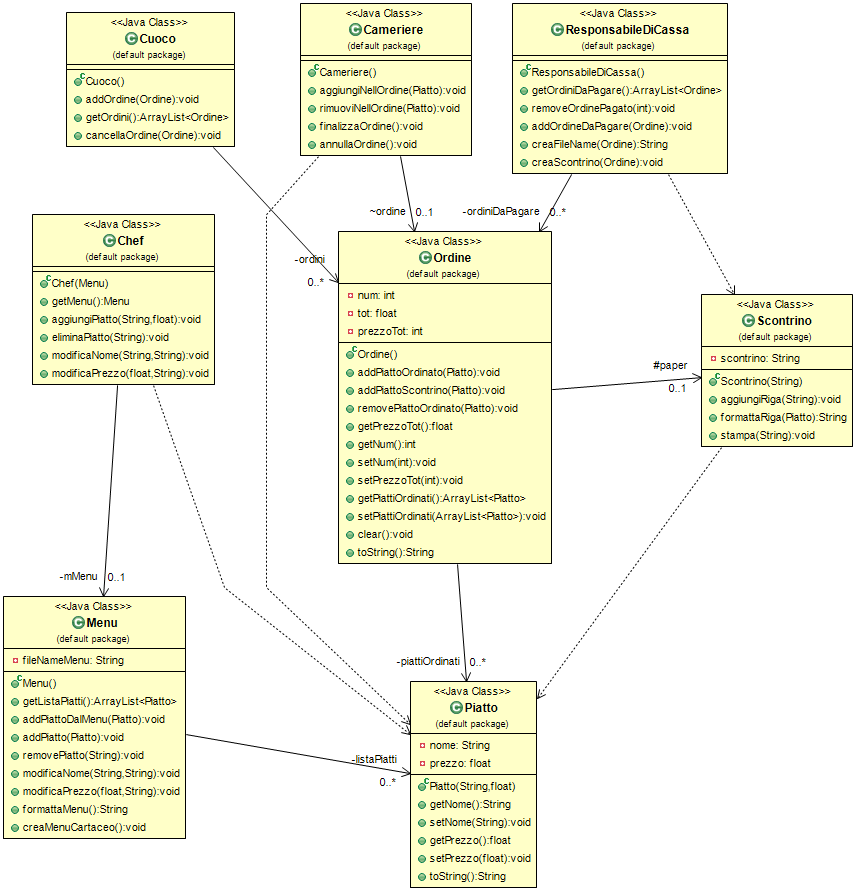
\includegraphics[width=\textwidth]{RestaurantManagerUML.png}
            
    \end{itemize}
    
    \newpage
    
    \section{Descrizione delle funzionalità}
    
    \subsection{Visualizzazione del menù iniziale}
    Il menu iniziale viene mostrato tramite un frame della classe JFrame all'avvio del programma, il quale è riempito con dei buttons della classe JButton che permettono di entrare nelle sezioni dei vari dipendenti, aggiornare il menu del ristorante, mostrato in primo piano nella finestra e uscire dal programma. Il menu del ristorante viene mostrato tramite un text pane della classe JTextPane il quale viene riempito all’avvio del programma con l’intero testo che si trova all’interno del file di testo ”MenuCartaceo.txt”.
    \\\\\\
    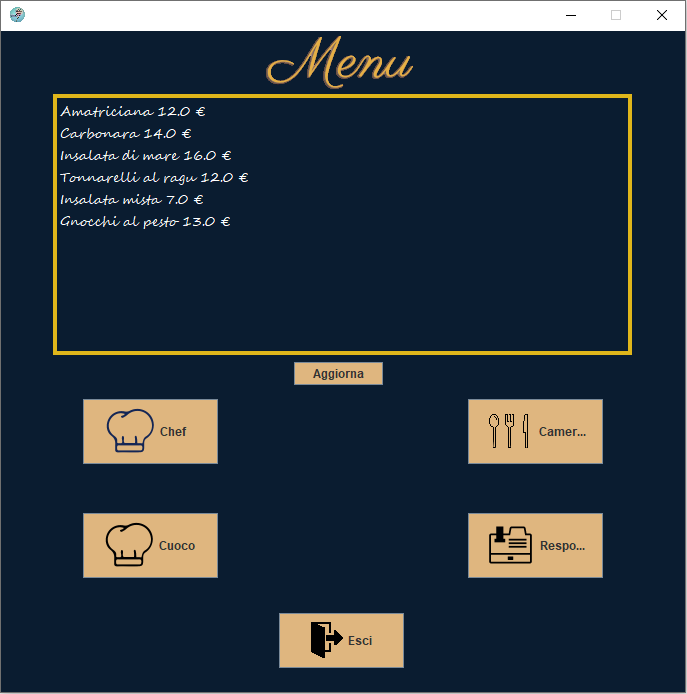
\includegraphics[width=\textwidth]{MenuPrincipale.png}
    \newpage
    
    \subsection{Sezione Chef}
    La sezione Chef gestisce il menu tramite un'istanza della classe stessa, attraverso la quale può intervenire sul file di testo "MenuCartaceo.txt" contenente i vari piatti che saranno poi disponibili all'interno del programma.
    \\\\\\
    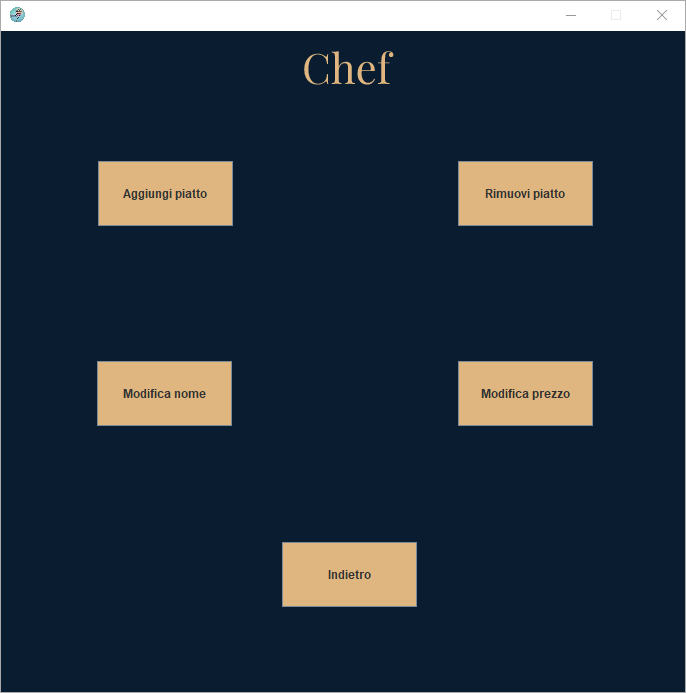
\includegraphics[width=\textwidth]{Chef.png}
    \\

    \begin{center}
        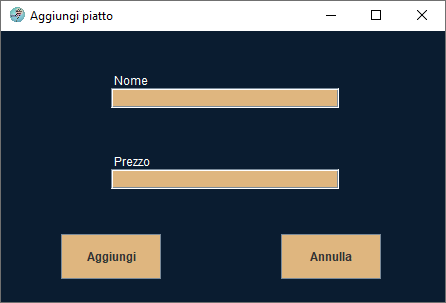
\includegraphics[scale=0.8]{ModificaChef.png}\\
        \caption{Le finestre dei restanti tre metodi sono analoghe}
    \end{center}
    
    %metti in una nuova pagina ogni sezione
    \subsection{Sezione Cameriere}
    La sezione Cameriere gestisce la creazione di ordini tramite un'istanza della classe stessa. In un ordine si possono aggiungere o rimuovere piatti e al termine del processo di modifica si può finalizzare l'ordine per mandarlo al Cuoco. Durante il processo si
    Prima di finalizzarlo il cameriere può mostrare la lista delle pietanze ordinate con il tasto "Controlla ordine".
    \\\\\\
    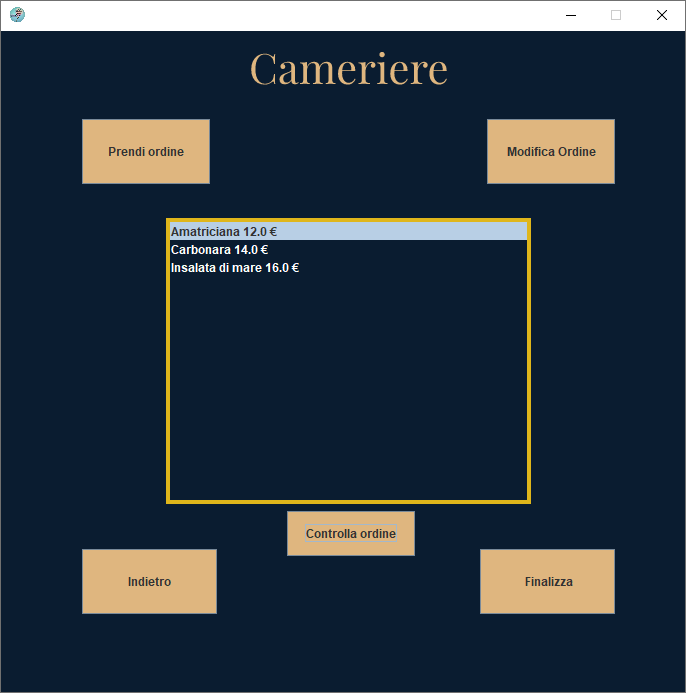
\includegraphics[width=\textwidth]{Cameriere.png}
    \\\\\\
    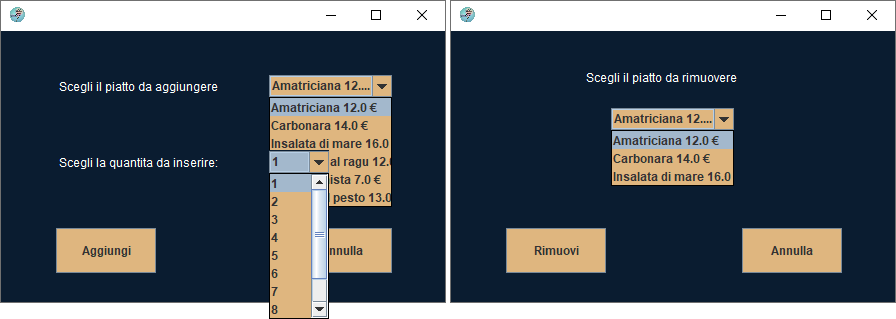
\includegraphics[width=\textwidth]{MetodiCameriere.png}
    
    %Nuova pagina
    \subsection{Sezione Cuoco}
    La sezione Cuoco gestisce gli ordini inviati da Cameriere rimuovendo i piatti all'interno dell'ordine selezionato uno per volta. All'interno dell'interfaccia grafica si possono selezionare i vari ordini e visualizzare i piatti da cucinare. Quando tutti i piatti in un ordine vengono evasi, l'ordine verrà mandato al responsabile di cassa.
    \\\\\\
    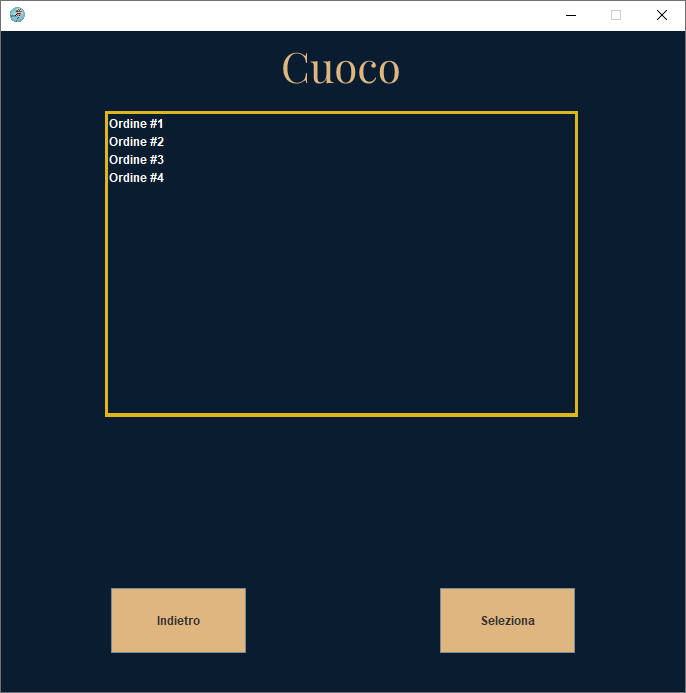
\includegraphics[width=\textwidth]{Cuoco.png}
    \\\\\\
    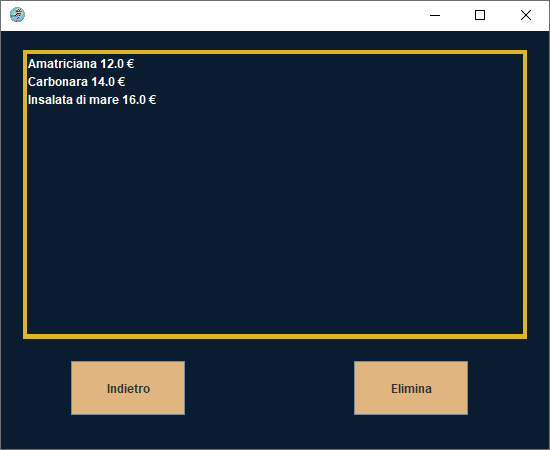
\includegraphics[scale=0.9]{MetodoCuoco.png}
    \\\\\\
    
    \newpage    
    \subsection{Sezione Responsabile di cassa}
    La sezione Responsabile di cassa gestisce gli ordini completati dal cuoco, permettendo la creazione dello scontrino.
    Dopo aver premuto il pulsante genera scontrino, questo verrà salvato in un file .txt nella directory principale del programma.
    \\\\\\
    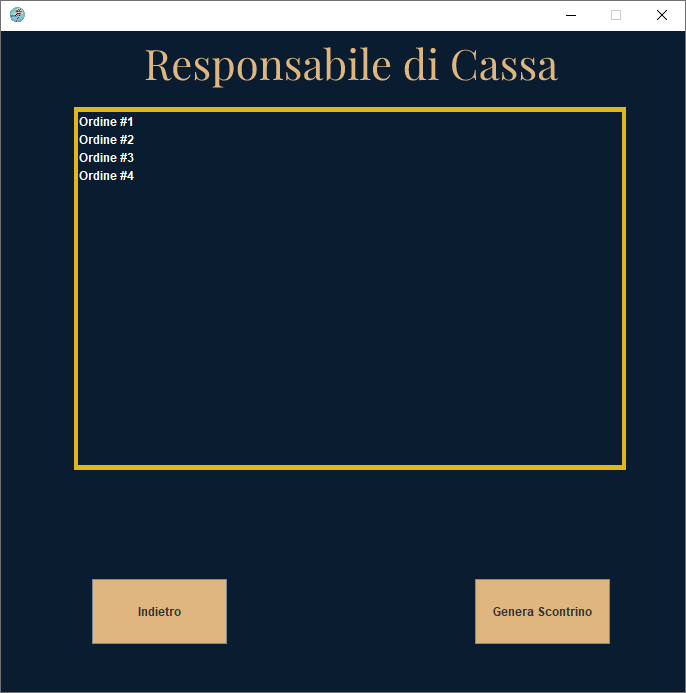
\includegraphics[width=\textwidth]{ResponsabileDiCassa.png}
    \\\\\\
    \begin{center}
        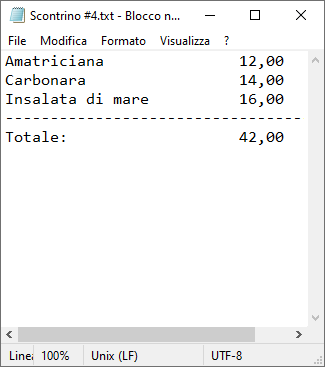
\includegraphics[scale=0.7]{Scontrino.png} \\
        \caption{Il file .txt generato dal Responsabile di Cassa}
    \end{center}
    
    \subsection{Schermate di Errore}
    Durante la normale esecuzione del programma si possono creare vari errori, i quali vengono presentati all'utente tramite schermate di errore.
    \\\\\\
    \begin{center}
        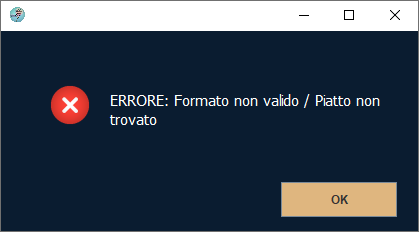
\includegraphics[scale=0.7]{Errore.png}\\
        \caption{Le varie schermate di errore sono simili tra loro}
    \end{center}
    
    \newpage
    
    \section{Referenti di sviluppo}
    Il programma è stato interamente sviluppato da Samuele Bella e Francesco De Persio in cooperazione.
    
\end{document}
